\subsection{المحول في الملاحقة}
في عام 
$2021$
بدأت تظهر أنظمة ملاحقة تستخدم المحول في بنيتها، سنذكر في هذه الفقرة بعض من تطبيقات المحول في مجال الملاحقة.
\newline
فمثلا استخدمت خوارزمية 
\textLR{TransT\cite{transformertracker}}
الطريقة الموضحة في الشكل 
\ref{fig:TransT}،
بداية تُستخدم شبكة 
\textLR{ResNet-50\cite{ResNet}}
لاستخلاص السمات من صورتي الغرض ومنطقة البحث، ومن ثم تستخدم كتلة انتباه ذاتي لكل من سمات الصورتين، مسماة في الورقة البحثية بـ
\textLR{ECA Ego-Context Augment Modules}
موضحة في المخطط اليسار من الشكل 
\ref{fig:TransT_Modules}.
ويتم دمج هذه السمات عبر كتلة انتباه تقاطعي تدعى بـ
\textLR{CFA Cross-Feature Augment Module}.
يتم الدمج عبر ثلاث مراحل موضحة في الشكل 
\ref{fig:TransT}
\begin{itemize}
	\item
	دمج خرج كتلة 
	\textLR{ECA}
	للغرض باعتبارها 
	\textLR{query}
	 ولمنطقة البحث باعتبارها
 	\textLR{key,value}.
 	\item
 	دمج بتبديل المداخل أي باعتبار سمات الغرض هي 
 	\textLR{key,value}
 	وسمات نافذة البحث هي 
	\textLR{query}.
 	\item
 	دمج الخرجين السابقين ضمن كتلة 
	\textLR{ECA}
	ثالثة.
\end{itemize}
مع إضافة ترميز مكاني إلى كل من 
\textLR{key,query}
في كل كتلة.
\newline

\begin{figure}[!h]
	\centerline{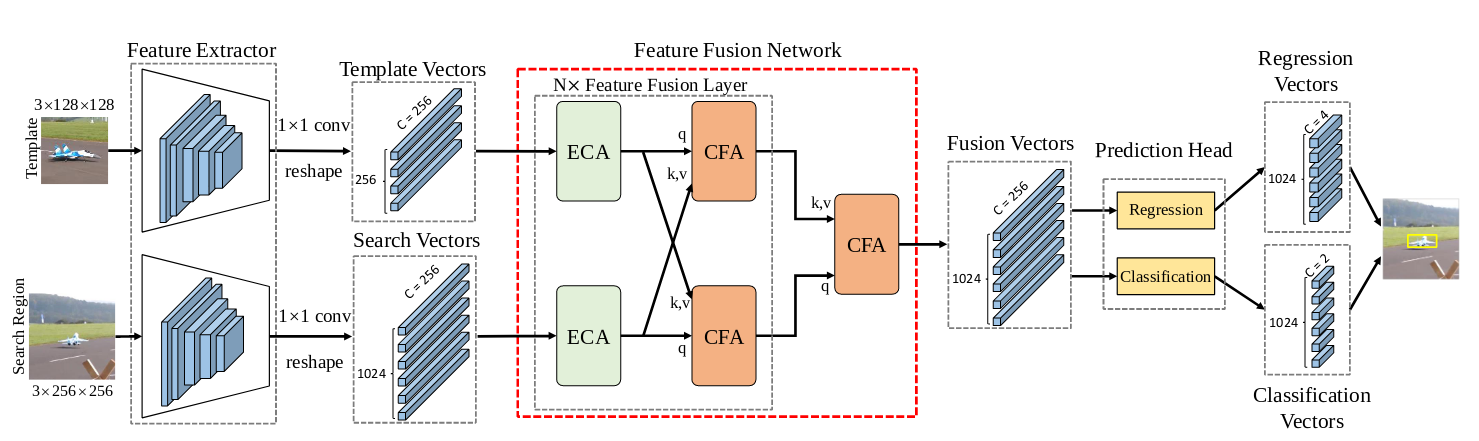
\includegraphics[width=\textwidth]{images/TransT}}
	\caption{
		\textRL{بنية خوارزمية الملاحقة}
		\textLR{TransT}
		\textLR{\cite{transformertracker}}}
	\label{fig:TransT}
\end{figure}

\begin{figure}[!h]
	\centerline{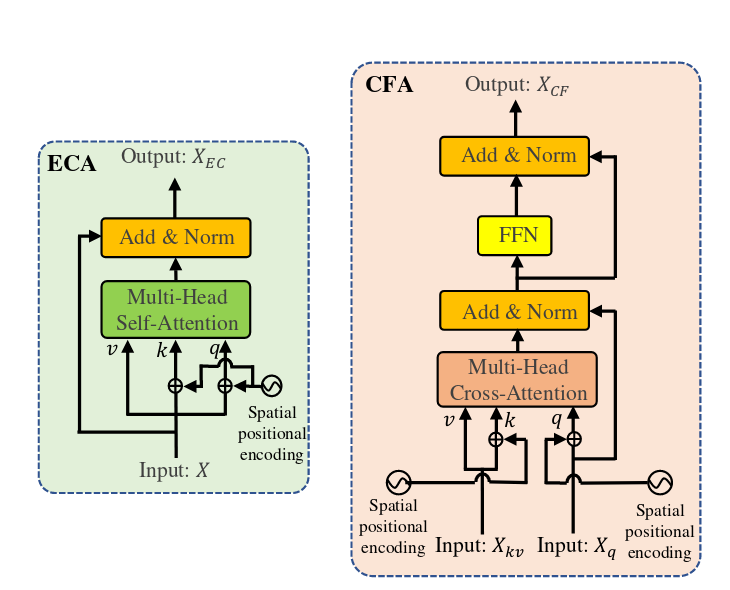
\includegraphics[scale=0.4]{images/TransT_ECA_CFA.png}}
	\caption{
		\textRL{بنية خوارزمية الملاحقة}
		\textLR{TransT}
		\textLR{\cite{transformertracker}}}
	\label{fig:TransT_Modules}
\end{figure}
كما أن خوارزمية الملاحقة
\textLR{TrTr\cite{TrTr}}
تستخدم بنية شبيهة ببنية المحول الأصلي كما يوضح الشكل 
\ref{fig:TrTr}،
بحيث يكون دخل المرمز هو سمات صورة الغرض الإبتدائية، ويطبق الانتباه الذاتي للتركيز على السمات المهمة. بينما يكون دخل مفكك الترميز هو سمات نافذة البحث ويطبق عليها تابع انتباه ذاتي، والدخل الثاني هو خرج المرمز (سمات الغرض المعدلة)، ويتم تطبيق تابع الانتباه التقاطعي بين الدخلين.
\begin{figure}[!h]
	\centerline{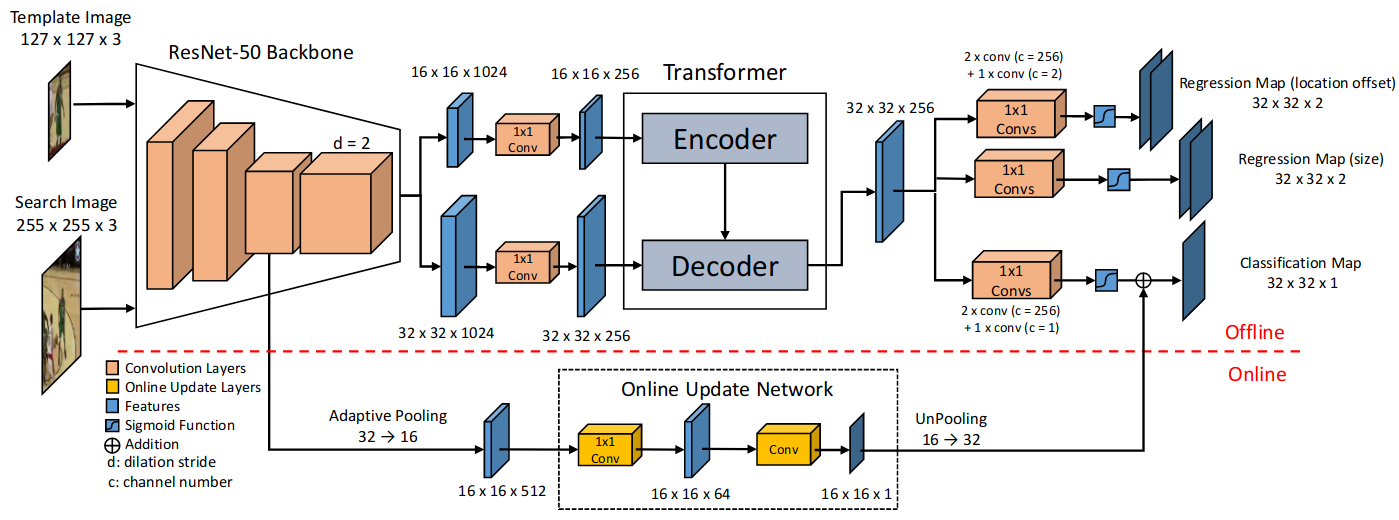
\includegraphics[width=\textwidth]{images/TrTr.png}}
	\caption{\textRL{بنية خوارزمية الملاحقة}
	\textLR{\cite{TrTr}}
	\textLR{TrTr}}
	\label{fig:TrTr}
\end{figure}
\newline
بالإضافة إلى خوارزميتي الملاحقة السابقتين فهناك خوارزمية الملاحقة 
\textLR{STARK\cite{Stark}},
وخوارزمية الملاحقة 
\textLR{SwinTrack\cite{swinTrack}}،
واللتان سيتم شرحهما بالتفصيل في الفصل القادم.
%وقد تم الاعتماد عليهما في البحث، وسيتم شرحهما بالتفصيل في الفصل القادم.
ويجب أن نلاحظ بمقارنة الخوارزميات الأربعة السابقة ببعضها بأن كل من 
\textLR{TransT\cite{transformertracker}}
و
\textLR{TrTr\cite{TrTr}}
تقوم بمعالجة سمات الغرض وسمات نافذة البحث على حدة ضمن توابع الانتباه، بينما في خوارزميات الملاحقة 
\textLR{SwinTrack\cite{swinTrack}}
و
\textLR{STARK\cite{Stark}}
كما سنرى لاحقاً،
فإنها تقوم بضم أشعة السمات للصورتين ضمن شعاع واحد، وتعتبره كدخل للمرمز.
\newline
هذا فيما يتعلق بخوارزميات الملاحقة لغرض واحد والتي تستخدم نموذج المحول ضمن بنيتها، وبمقارنة هذه الخوارزميات بسابقتها والتي لا تستخدم المحول، فنلاحظ كما يوضح الشكل
\ref{fig:comapre}،
والذي يقارن عدة خوارزميات ملاحقة حديثة من ناحية الأداء والسرعة على مجموعة المعطيات الخاصة بالملاحقة 
\textLR{LaSOT\cite{Lasot}}،
بأن خوارزميات الملاحقة التي تستخدم المحول حققت أفضل أداء وسرعة مقارنةً بغيرها من الخوارزميات، وهذا ماشجعنا على اعتمادها في البحث.
وبمقارنة الخوارزميات الأربعة السابقة بالنسبة لبعضها فنلاحظ من الجدول 
\ref{table:compare__trans_trackers}،
والذي يقارن هذه الخوارزميات من أجل مجموعة المعطيات 
\textLR{LaSOT\cite{Lasot}}،
بأن أفضل أداء حققته خوارزمية 
\textLR{SwinTrack\cite{swinTrack}}، 
يليها خوارزمية 
\textLR{STARK\cite{Stark}}،
وبسبب تفوق خوارزمية 
\textLR{SwinTrack\cite{swinTrack}}
في الأداء والسرعة، قررنا أن نعتمدها في بحثنا.
\begin{figure}[!h]
	\centerline{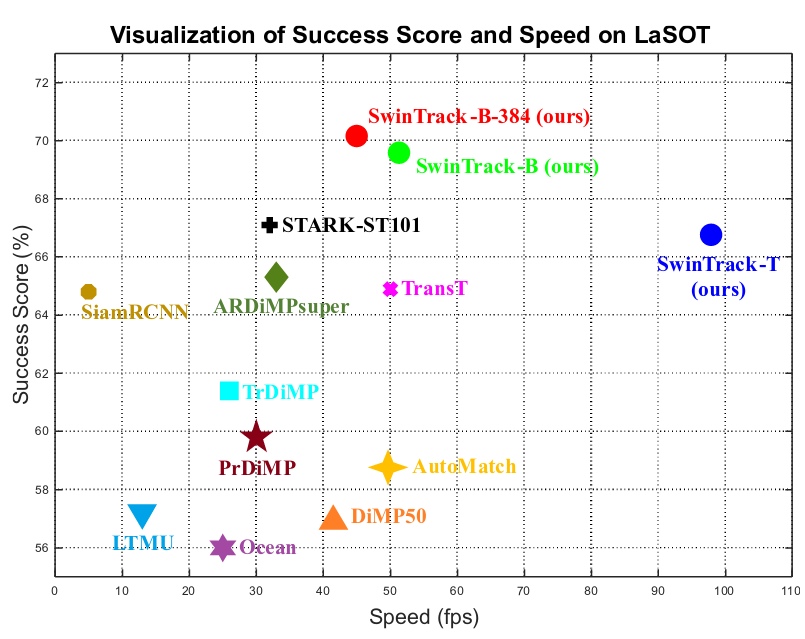
\includegraphics[width=0.6\textwidth]{images/transformerInTrackingComapre.png}}
	\caption{
		\textRL{مقارنة بين بعض الخوارزميات التي تستخدم المحول مع خوارزميات الملاحقة الأخرى
			 من ناحية السرعة و الأداء على مجموعة المعطيات}
		 \textLR{LaSOT\cite{Lasot}}
		\textLR{\cite{swinTrack}}
		}
	\label{fig:comapre}
\end{figure}

\begin{table}[!h]
	\centering
	\begin{tabular}{c c c c c c c} 
		\hline
		\textLR{Tracker} & \textLR{AUC}\% & \textLR{Normalized Precision} & \textLR{Precision}&\textLR{Year}\\ [0.5ex] 
		\hline\hline
		\textLR{SwinTrack-B-384} &$70.2$&$78.4$&$75.3$&$2021$\\
		\textLR{STARK} & $67.1$ & $77.0$ &&$2021$\\ 
		\textLR{TransT} &$64.9$ & $73.8$ & $69.0$&$2021$\\
		\textLR{TrTr} & $55.1$ &&&$2021$&\\[1ex] 
		\hline
	\end{tabular}
	\caption{
		\begin{footnotesize}
		\textRL{مقارنة بين خوارزميات الملاحقة السابقة}
		\textRL{من أجل معطيات التدريب}
		\textLR{LaSOT\cite{Lasot}}
		\end{footnotesize}}
	\label{table:compare__trans_trackers}
\end{table}
أما فيما يتعلق بالملاحقة لعدة أغراض فهناك خوارزمية 
\textLR{TrackFormer\cite{TrackFormer}}
والتي استخدمت بنية محول مشابهة لخوارزمية
\textLR{TrTr\cite{TrTr}},
بينما استخدمت خوارزمية
\textLR{TransTrack\cite{TransTrack}}
سمات الإطار الحالي والإطار السابق كدخل للمرمز مع استخدام كتلتي مفكك ترميز،
دخل مفكك الترميز هو
\textLR{object query} 
قابلة للتدريب، وذلك كما في خوارزمية 
\textLR{DETR\cite{DETR}}
المشروحة في الفقرة 
\ref{section:detr}.